\documentclass{article}


% if you need to pass options to natbib, use, e.g.:
%     \PassOptionsToPackage{numbers, compress}{natbib}
% before loading svrhm_2022


% ready for submission
\usepackage{svrhm_2022}


% to compile a preprint version, e.g., for submission to arXiv, add add the
% [preprint] option:
%     \usepackage[preprint]{svrhm_2022}


% to compile a camera-ready version, add the [final] option, e.g.:
%     \usepackage[final]{svrhm_2022}


% to avoid loading the natbib package, add option nonatbib:
%    \usepackage[nonatbib]{svrhm_2022}


\usepackage[utf8]{inputenc} % allow utf-8 input
\usepackage[T1]{fontenc}    % use 8-bit T1 fonts
\usepackage{graphicx}
\usepackage{hyperref}       % hyperlinks
\usepackage{url}            % simple URL typesetting
\usepackage{booktabs}       % professional-quality tables
\usepackage{amsfonts}       % blackboard math symbols
\usepackage{nicefrac}       % compact symbols for 1/2, etc.
\usepackage{microtype}      % microtypography
\usepackage{xcolor}         % colors
\usepackage{multirow}
\usepackage{subcaption}
\usepackage{amssymb,amsmath,array}

\title{Population Coding Can Greatly Improve Performance of Neural Networks: A Comparison}


% The \author macro works with any number of authors. There are two commands
% used to separate the names and addresses of multiple authors: \And and \AND.
%
% Using \And between authors leaves it to LaTeX to determine where to break the
% lines. Using \AND forces a line break at that point. So, if LaTeX puts 3 of 4
% authors names on the first line, and the last on the second line, try using
% \AND instead of \And before the third author name.

\author{%
Rebecca K\"ohler\\
Institut für Neuro- und Bioinformatik\\
Universität zu Lübeck\\
Lübeck, 23562 \\
\texttt{rebecca.koehler@student.uni-luebeck.de} \\
% examples of more authors
\And
Hans-Oliver Hansen\thanks{Equal contributions} \\
Institut für Neuro- und Bioinformatik\\
Universität zu Lübeck\\
Lübeck, 23562 \\
\texttt{hohansen@inb.uni-luebeck.de} \\
% examples of more authors
\And
Marius Jahrens$^*$ \\
Institut für Neuro- und Bioinformatik\\
Universität zu Lübeck\\
Lübeck, 23562 \\
\texttt{jahrens@inb.uni-luebeck.de} \\
% examples of more authors
\And
Thomas Martinetz \\
Institut für Neuro- und Bioinformatik\\
Universität zu Lübeck\\
Lübeck, 23562 \\
\texttt{martinetz@inb.uni-luebeck.de} \\
% examples of more authors
  % Coauthor \\
  % Affiliation \\
  % Address \\
  % \texttt{email} \\
  % \AND
  % Coauthor \\
  % Affiliation \\
  % Address \\
  % \texttt{email} \\
  % \And
  % Coauthor \\
  % Affiliation \\
  % Address \\
  % \texttt{email} \\
  % \And
  % Coauthor \\
  % Affiliation \\
  % Address \\
  % \texttt{email} \\
}


\begin{document}


\maketitle


\begin{abstract}
  Artificial neural networks oftentimes operate on continuous inputs. 
While biological neural networks usually represent information through the activity of a population of neurons, 
the inputs of an artificial neural network are typically provided as a list of scalars. 
As the information content of each of the input scalars depends heavily on the problem domain, 
representing them as individual scalar inputs, irrespective of the amount of information they contain, may prove to be suboptimal for the network. 
We therefore compare and examine four different population coding schemes and demonstrate that 
applying population coding to information rich, low dimensional inputs can vastly improve a network's performance.
\end{abstract}


% !TEX root = ../svrhm.tex
\section{Introduction}

Recently, multiple publications have shown that it is beneficial for neural networks to encode continuous inputs
as vector encodings \cite{mildenhall2020nerf}\cite{jahrens2020solving}, also known as population coding. 
For that, the scalar components of the network input would be represented as vectors such that the value of a scalar will not be defined by the extend of a single stimulus, but by the pattern in the vector.

In nature this principle can be observed in the activation patterns that represent joint position or eye position as well as an organism's location in space, i.e. grid cells as described by \cite{haftin2005gridcells}. For different purposes different encoding schemes are used. These can be distinguished by the neurons employing unimodal or multimodal activation characteristics. In this paper we explore examples for both types of encoding schemes. 

For a closed set of discrete values, this has been done for a while in the form of learned embeddings, e.g. in language models with a fixed dictionary \cite{devlin2019bert}.
For an open set of discrete values, a similar concept can be found in position encodings \cite{vaswani2017transformer}. 
However, position encodings are usually only applied to the positional information of elements in a sequence or tensor, rather than to encode the scalar values of the input sample.

The benefit of applying population coding to neural network inputs has been demonstrated not only for information rich, independent scalars like cartesian coordinates \cite{mildenhall2020nerf}, 
but also highly correlated scalars like pixel values in images \cite{jahrens2020solving}. 
A more thorough analysis of existing approaches would therefore aid in determining the usefulness and potential pitfalls of population coding in current neural networks.

We compare four population coding schemes and examine their utility in a regression setting. 
We show that population coding can drastically improve a model's performance in a way that cannot be explained by the increased network depth or number of parameters.
% !TEX root = ../svrhm.tex
\section{Related work}
Population coding was successfully used in several publications to increase a network's performance. 
The authors of \cite{mildenhall2020nerf} used Positional Encoding on a camera pose vector, a five dimensional input vector $(x,y,z,\theta, \phi)$ with spacial coordinates $x$, $y$ and $z$ as well as orientation $\theta$ and $\phi$ to learn the corresponding RGB-values on the line of sight.
Encoding the low-dimensional inputs was essential to achieve good results on their regression problem. 

In \cite{jahrens2020solving} another population coding scheme called Magnitude Encoding was employed to get a new representation of the individual intensity values of grey scale images. 
The model processes multiple images per sample and uses late fusion, so the improved performance may be attributed to improved information retention.
The input encoding turned out to be crucial to solve certain tasks pertaining to color. 

% In a work focused on optimizing the encoding of coordinates Fourier Feature Mapping \cite{tancik2020fourier} was introduced. 
% The authors have shown the high impact of their encoding scheme on the capacity of MLPs to learn high frequency dependencies between input and output. 
The authors of \cite{tancik2020fourier} introduced Fourier Feature Mapping and demonstated the high impact of their encoding scheme on the capacity of MLPs to learn high frequency dependencies between input and output. 

% Each of these approaches lead to huge improvements in the networks' comprehension of (scalar) data.
% !TEX root = ../svrhm.tex
\section{Population coding}
%Die 4 Varianten benennen, Formeln angeben, Parameter definieren (Sigma, M) (+Referenzen)
%\textit{Anmerkung: Für eine Verallgemeinerung auf Inputgroesse $d$ muessen hier nochmal die Formeln angepasst werden, da wir in der Bachelorarbeit mit $d=2$ gearbeitet haben.}
%This paper looks at four different methods of population coding in order to compare them. These four methods are described below. 
Across all encodings the input values are assumed to be in the range -1 to 1. 
The resulting encoded vector is a concatenation of the encoded components. The visualizations can be found in the appendix \ref{subsecPlots}.

\subsection{Positional Encoding}
For a multimodal example we explore Positional Encoding (PE) as described in \cite{mildenhall2020nerf} uses a combination of sine and cosine functions with exponential frequencies to encode the given input values:
\begin{align*}
    f(x) = [sin(2^0\pi x),\ldots,sin(2^{L-1}\pi x),cos(2^0\pi x),\ldots,cos(2^{L-1}\pi x)]
\end{align*}
for each input scalar $x$. 

\subsection{Fourier Feature Mapping}
Fourier Feature Mapping (FFM) was introduced in \cite{tancik2020fourier}. In contrast to PE, the components are not encoded individually but instead the input vector is transformed via random linear operation:
\begin{align*}
    f(\textbf{p}) = [a_1 sin(2\pi\textbf{b}_1^T\textbf{p}),\ldots,a_L sin(2\pi\textbf{b}_L^T\textbf{p}),a_1 cos(2\pi\textbf{b}_1^T\textbf{p}),\ldots,a_L cos(2\pi \textbf{b}_L^T\textbf{p})].
\end{align*}

In this paper we use $a_k=1$ for all $k$ in order to get a direct comparison between FFM and other encoding methods. The random vectors $\textbf{b}_i$ are drawn independently from a standard normal distribution.

\subsection{Tent Encoding}
For a unimodal example we explore Tent Encoding (TE) by the authors of \cite{jahrens2020solving} is based on the tent mapping.
    \[t(x) = \begin{cases} x+1 & x \in [-1,0] \\ -x+1 & x \in (0,1]\\ 0 & \text{else} \end{cases}\]
In addition to translations $t(\cdot-a)$, TE uses different slopes $m$ that can be adjusted:
\begin{align*}
    &f(x) =\left[t\left(m\cdot(x-\mu_0)\right), t\left(m\cdot(x-\mu_1)\right),\ldots,t\left(m\cdot(x-\mu_{L-1})\right)\right]\\&\text{with }\mu_i=\frac{2\cdot i}{L-1}-1\quad\forall\ i=0,\ldots,L-1.
\end{align*}

\subsection{Magnitude Encoding}
Magnitude Encoding (ME) as described in \cite{jahrens2020solving} uses Gaussian bell curves $g(x)=\exp(-x^2/(2\sigma^2))$. Each input component is encoded via
\begin{align*}
    &f(x) =\left[g\left(x-\mu_0\right), g\left(x-\mu_1\right),\ldots,g\left(x-\mu_{L-1}\right)\right]\\&\text{with }\mu_i=\frac{2\cdot i}{L-1}-1\quad\forall\ i=0,\ldots,L-1.
\end{align*}
% !TEX root = ../svrhm.tex
\section{Experiments}
\subsection{Experiment design}
%Architektur, Inputs, Outputs, Beschreibung Lernen der Koordinaten->Pixelwert Zuordnung, Lossfunktion
%Referenz zu analogem Experiment in FFM Paper
Using a similar experiment setup as described in \cite{tancik2020fourier}, we analyse the impact of applying population coding on the input of a neural network by training the network on a single image. 
It takes the image coordinates as inputs and performs a regression on the corresponding color values. 
We use a multilayer perceptron (MLP) with four hidden layers, each of size 256, and ReLU activations. 
The output consists of 3 channels with sigmoid activations for the RGB-values. 
The Mean Squared Error (MSE) is used as loss function. 
The input image consists of 12000 pixels of which 90\% are used as training data and 10\% as test data. 
The MLP is trained over 12000 epochs.

The input coordinates are scaled to $[-1,1]$. Five different population sizes $d \in \{16, 32, 64, 128, 256\}$ are examined. The network's output images are evaluated visually as well as quantitatively by the MSE.

\begin{figure}[h]
  \begin{minipage}{.48\textwidth}
    \centering
    \subcaptionbox{Input image\label{input}}
    {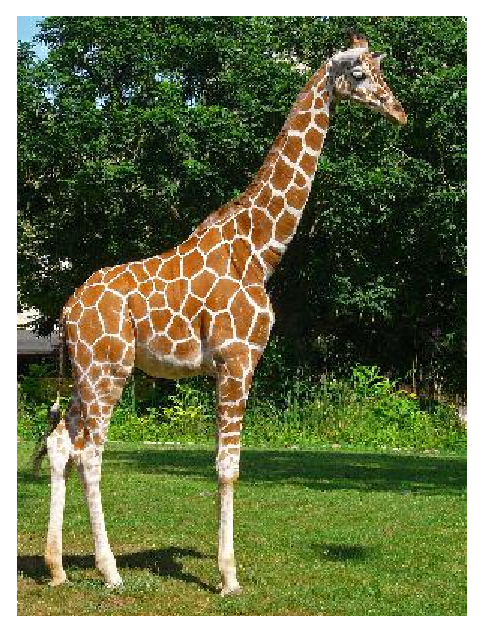
\includegraphics[width=0.45\textwidth]{Bilder/Giraffe/Giraffe_verkleinert_400x300.eps}}
    %\label{input}
    \subcaptionbox{No encoding\label{noEnc}}
    {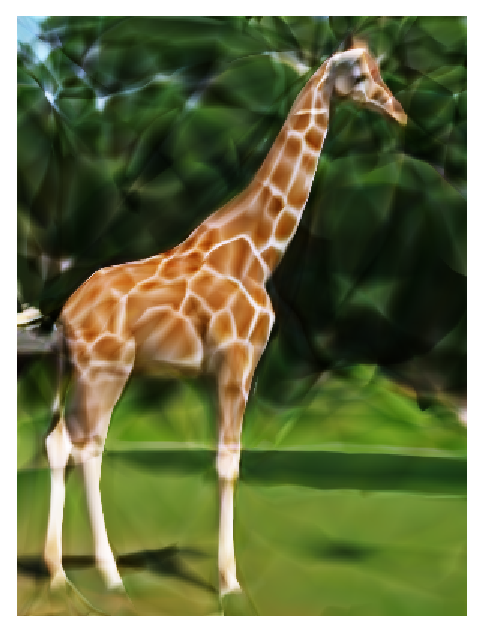
\includegraphics[width=0.45\textwidth]{Bilder/Giraffe/image_result_scale12000_indim2_lr0.003333.eps}}
      %\label{noEnc}
\caption{Reference image \cite{giraffeonline} and reconstructed image without encoding}
\label{InputNoEnc}
\end{minipage}\quad
\begin{minipage}[c]{.25\textwidth}
  \centering
  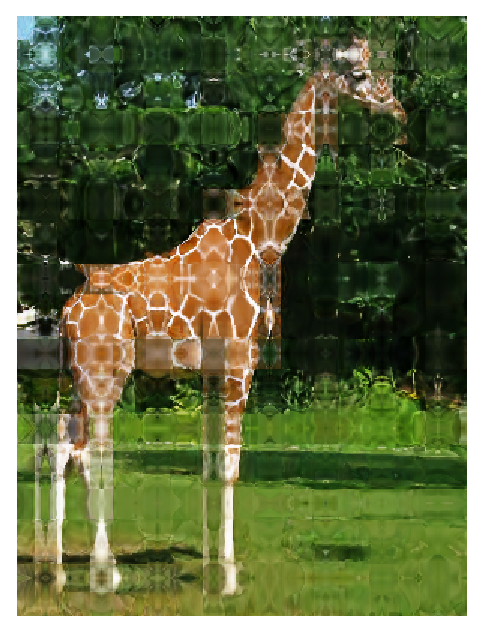
\includegraphics[width=\textwidth]{Bilder/Giraffe/spiegelungen_image_result_tent12000_indim16_lr0.0125_m5.eps}
  \caption{TE artifacts, $d$=16, $m$=5}
  \label{TEartefact}
\end{minipage}

\end{figure}


\begin{table}
  \caption{Minimum training and test loss achieved within 12000 epochs of learning for different encodings with dimension $d$.}
  \label{train_test_losses}
  \vspace{0.2cm}
  \centering
  \begin{tabular}[H]{cccc}
    \toprule
  \textbf{encoding} & $\boldsymbol{d}$ &\textbf{train loss} &\textbf{test loss}\\
  \midrule
  \textbf{none} & 2 & 0.016 & 0.018 \\
  \midrule
  \multirow{2}{*}{\textbf{FFM}} & 16 & 0.0086 & 0.0160 \\
    & 256 & 0.0057 & 0.0153 \\
  \midrule
  \multirow{2}{*}{\textbf{PE}} & 16 & 0.0063 & 0.0156 \\
  & 256 & 0.0004 & 0.0298 \\
  \midrule
  \multirow{2}{*}{\textbf{TE}} & 16 & 0.0092 & 0.0156 \\
    & 256 & 0.0005 & 0.0177 \\
  \midrule
  \multirow{2}{*}{\textbf{ME}} & 16 & 0.0111 & 0.0158 \\
  & 256 & 0.0007 & 0.0170 \\
  \bottomrule
  \end{tabular}
\end{table}

\begin{figure}
  \begin{subfigure}{0.5\textwidth}
    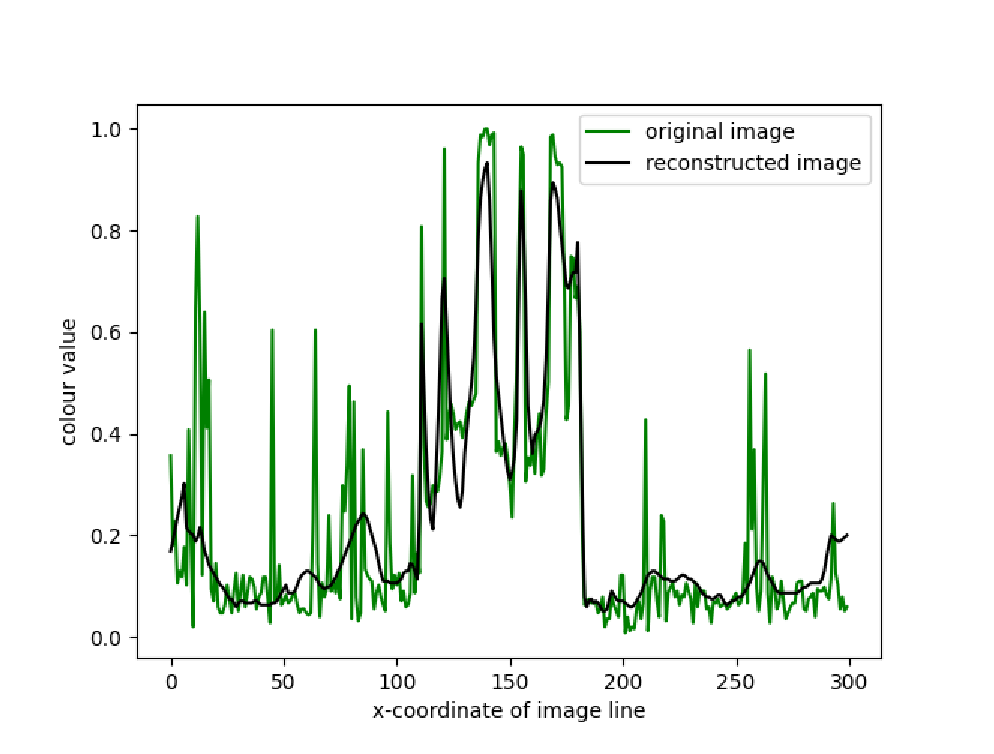
\includegraphics[width=.85\textwidth]{Bilder/Zeilenanalyse/lines_scale_channel1.eps}
   \end{subfigure}
   \begin{subfigure}{0.5\textwidth}
  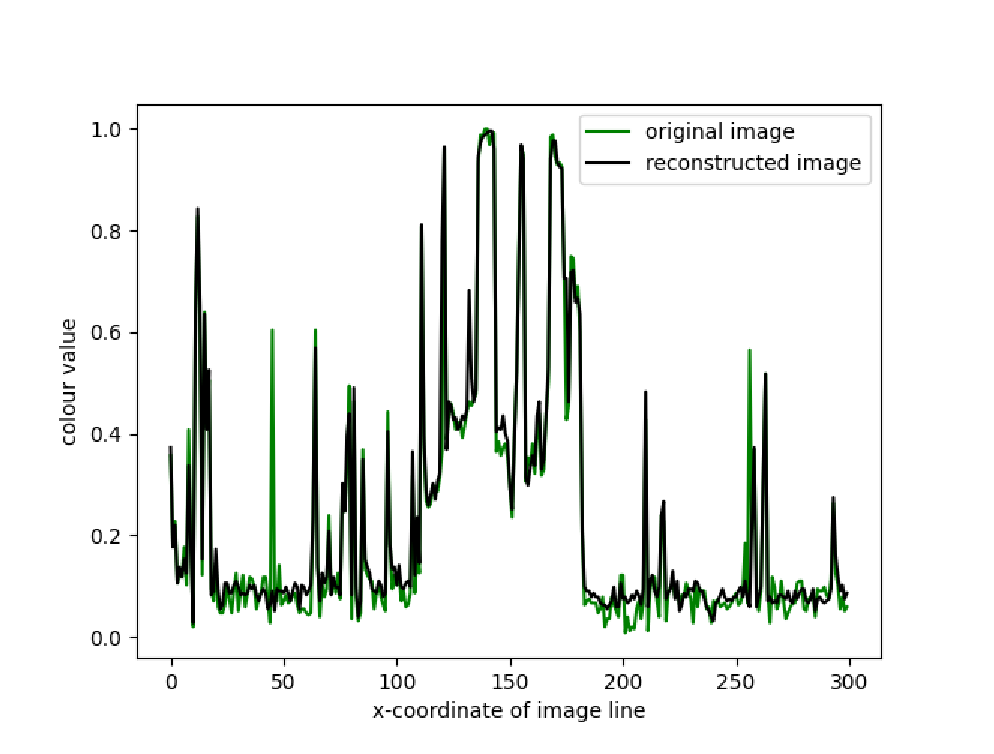
\includegraphics[width=.85\textwidth]{Bilder/Zeilenanalyse/lines_tent_channel1.eps}
  \end{subfigure}
  \caption{Values of green channel in row 150, top: no encoding, bottom: TE.}
  \label{lineAnalysis}
  % \caption{Reference image \cite{giraffeonline}, its reconstruction by an MLP without input encoding and a failed reconstruction with TE}
  % \label{RefNoEncTE}
\end{figure}

\subsection{Encodings}
In figure \ref{outputImages} the output images are visualized for each encoding. By only passing the two-dimensional coordinates as input, the MLP is unable to learn high-frequency dependencies (figure \ref{noEnc}). 
%The lowest train loss which is achieved within the 12000 epochs is $0.0159$ and the lowest test loss $0.018$. 
The utilisation of each encoding leads to higher resolution of the output. Using any encoding with population size $d = 16$ already yields a significant improvement in the reconstructed image. Increasing the population size enhances the output's image quality further. Population sizes beyond $d = 256$ offer diminishing returns. When using TE, the best results are achieved when setting $m$ to a quarter of the input dimension. Here, the output image of $d = 256$ with $m = 64$ can hardly be distinguished from the input image. Comparable results are achieved with ME and $d = 256$. 

In table \ref{train_test_losses}, the minimum training and test loss are shown. The results correlate with the visual observations. The use of each encoding, even with only 16 dimensions, leads to lower training losses. Notably, the test loss with $d=16$ in each encoding is better than the training loss with no encoding.

%Starting with $d = 16$, an improvement of the learning ability of the MLP can be observed. By the increase of $d$, the MLP performs better.


\begin{figure}[!h]
    
    \begin{subfigure}{.25\textwidth}
      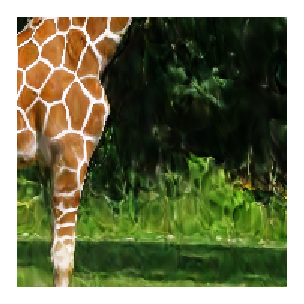
\includegraphics[width=\textwidth]{Bilder/Giraffe/Bildausschnitte/image_result_fourier12000_indim16_lr0.0125.eps}
      \caption{FFM, $d$=16}
      \label{FFM16}
    \end{subfigure}\hfil
    \begin{subfigure}{.25\textwidth}
      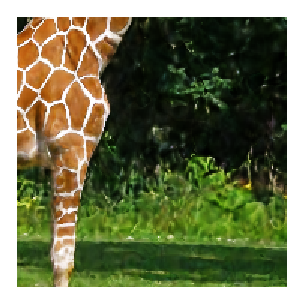
\includegraphics[width=\textwidth]{Bilder/Giraffe/Bildausschnitte/image_result_positional12000_indim16_lr0.003333.eps}
      \caption{PE, $d$=16}
      \label{PE16}
    \end{subfigure}\hfil
    \begin{subfigure}{.25\textwidth}
      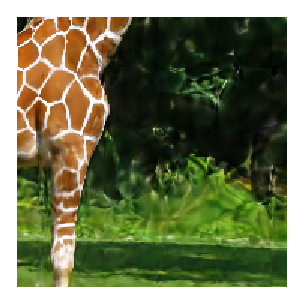
\includegraphics[width=\textwidth]{Bilder/Giraffe/Bildausschnitte/image_result_tent12000_indim16_lr0.006667_m4.eps}
      \caption{TE, $d$=16}
      \label{TE16}
    \end{subfigure}\hfil
    \begin{subfigure}{.25\textwidth}
      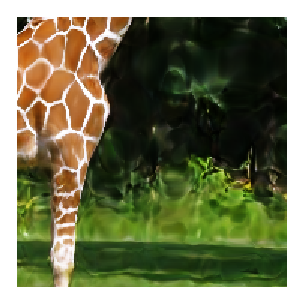
\includegraphics[width=\textwidth]{Bilder/Giraffe/Bildausschnitte/image_result_magnitude12000_indim16_lr0.006667_sigma0.1.eps}
      \caption{ME, $d$=16}
      \label{ME16}
    \end{subfigure}\hfil

  %256 dimensions
  
  \begin{subfigure}{.25\textwidth}
  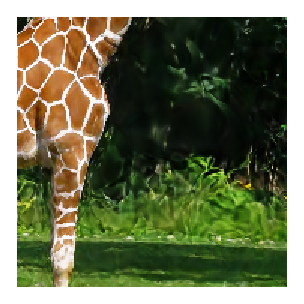
\includegraphics[width=\textwidth]{Bilder/Giraffe/Bildausschnitte/image_result_fourier12000_indim256_lr0.006667.eps}
  \caption{FFM, $d$=256}
  \label{FFM256}
  \end{subfigure}\hfil
  \begin{subfigure}{.25\textwidth}
    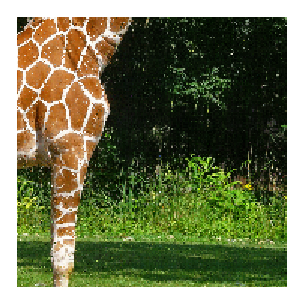
\includegraphics[width=\textwidth]{Bilder/Giraffe/Bildausschnitte/image_result_positional12000_indim256_lr0.003333.eps}
    \caption{PE, $d$=256}
    \label{PE256}
  \end{subfigure}\hfil
  \begin{subfigure}{.25\textwidth}
    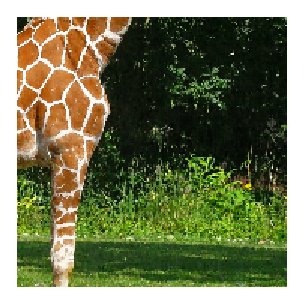
\includegraphics[width=\textwidth]{Bilder/Giraffe/Bildausschnitte/image_result_tent12000_indim256_lr0.006667_m64.eps}
    \caption{TE, $d$=256}
    \label{TE256}
  \end{subfigure}\hfil
  \begin{subfigure}{.25\textwidth}
    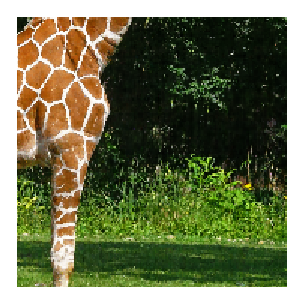
\includegraphics[width=\textwidth]{Bilder/Giraffe/Bildausschnitte/image_result_magnitude12000_indim256_lr0.006667_sigma0.007.eps}
    \caption{ME, $d$=256}
    \label{ME256}
  \end{subfigure}\hfil
  %\begin{subfigure}{.33\textwidth}
  %  \includegraphics[width=\textwidth]{}
  %  \caption{PE artefacts, $d$=256}
  %  \label{PEartefact}
  %\end{subfigure}\hfil
  
\caption{Best output images of each encoding with population sizes $d=16$ and $d=256$, standard deviation $\sigma$ for (d) 0.1 and (h) 0.007, and slope $m$ for (c) 4 and (g) 64.}
\label{outputImages}
\end{figure}

%Bildreihe mit 16-dim und 256-dim für alle Kodierungen (+ Originalbild + Ergebnis ohne Kodierung)
%(in Bildunterschrift ansprechen, dass jeweils optimales Sigma + M gewaehlt wurde)

\subsection{Single-line analysis}
For further analysis, the color values of a single line in the target and generated image are compared in figure \ref{lineAnalysis} with population size $d=256$. Without encoding, the values are approximated poorly and peaks are not represented well. In contrast with TE, the MLP is able to learn higher frequency dependencies.


% \subsection{Local MSE-Loss}
% \label{LocalMSE}
% To localize the contribution to the overall reconstruction loss the mean squared error is calculated over a sliding $10\times10$-window on a single channel. The resulting loss map is shown in figure \ref{MSE256}.
% % \begin{figure}
% %   \begin{subfigure}{.25\textwidth}
% %     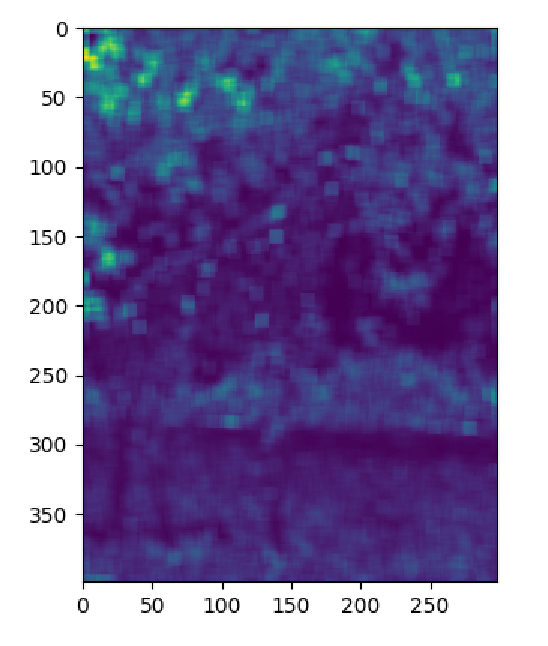
\includegraphics[width=\textwidth]{Bilder/MSE_Bilder/cropped/kernel10_positional_16_0.003_m0_G.eps}
% %     \caption{PE}
% %     \label{MSE16PE}
% %   \end{subfigure}\hfil
% %   \begin{subfigure}{.25\textwidth}
% %     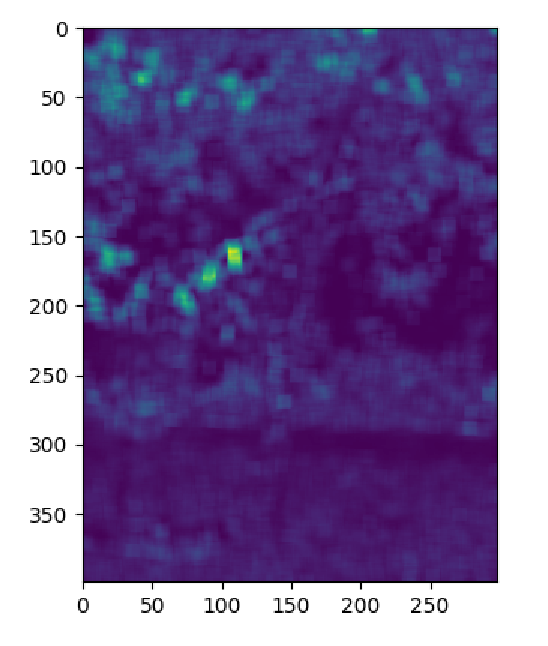
\includegraphics[width=\textwidth]{Bilder/MSE_Bilder/cropped/kernel10_fourier_16_0.01_G.eps}
% %     \caption{FFM}
% %     \label{MSE16FFM}
% %   \end{subfigure}\hfil
% %   \begin{subfigure}{.25\textwidth}
% %     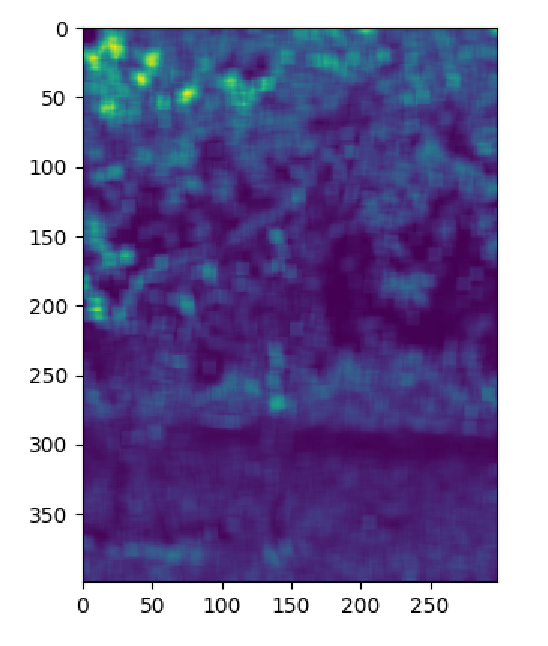
\includegraphics[width=\textwidth]{Bilder/MSE_Bilder/cropped/kernel10_tent16_m4_0.00667_G.eps}
% %     \caption{TE}
% %     \label{MSE16TE}
% %   \end{subfigure}\hfil
% %   \begin{subfigure}{.25\textwidth}
% %     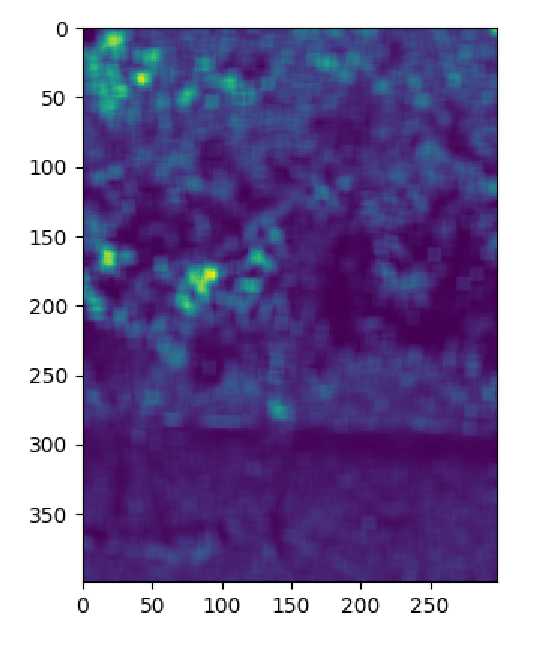
\includegraphics[width=\textwidth]{Bilder/MSE_Bilder/cropped/kernel10_magnitude_16_0.007_m0.05_G.eps}
% %     \caption{ME}
% %     \label{MSE16ME}
% %   \end{subfigure}\hfill
% %   \caption{Local MSE-Loss for $d=16$, green channel, brighter colors represent larger values}
% %   \label{MSE16}
% % \end{figure}

% While each of the encoding approaches leads to better image reconstruction than no enconding at all. The image background exhibits a higher loss than objects in the foreground. This may be attributed to the background features having higher entropy, i.e. higher information content. Another explanation is the occurrence of higher frequency features. PE and FFM lead to better resulting images than TE and ME.

% \begin{figure}
%   \begin{subfigure}{.25\textwidth}
%     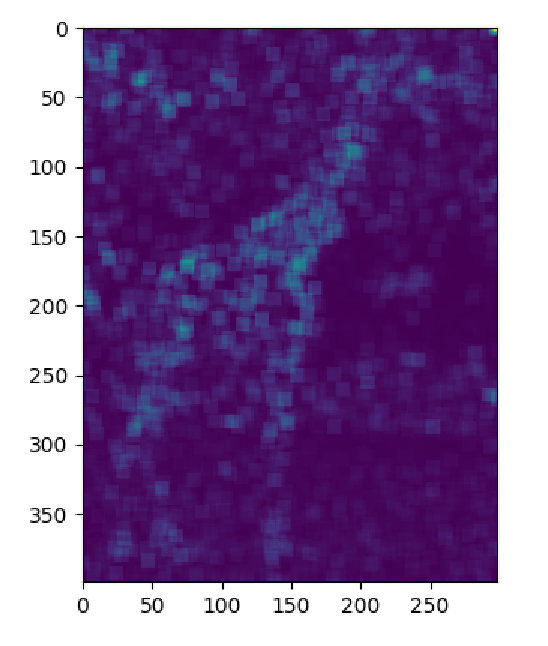
\includegraphics[width=\textwidth]{Bilder/MSE_Bilder/cropped/kernel10_positional_256_0.003_m0_G.eps}
%     \caption{PE}
%     \label{MSE256PE}
%   \end{subfigure}\hfil
%   \begin{subfigure}{.25\textwidth}
%     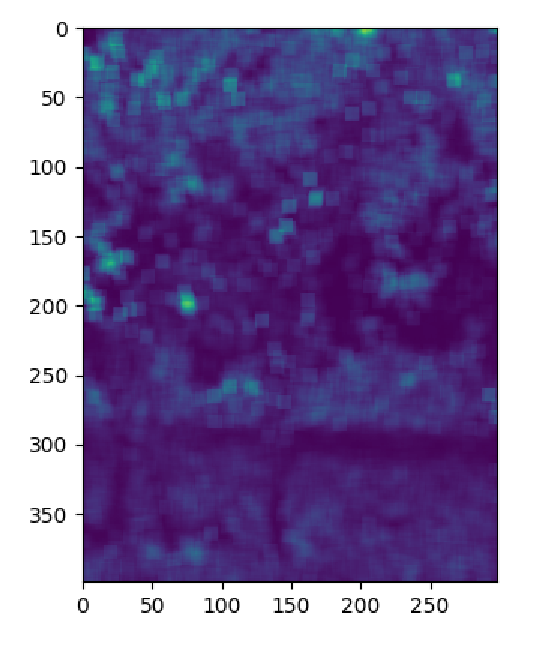
\includegraphics[width=\textwidth]{Bilder/MSE_Bilder/cropped/kernel10_fourier_256_0.01_G.eps}
%     \caption{FFM}
%     \label{MSE256FFM}
%   \end{subfigure}\hfil
%   \begin{subfigure}{.25\textwidth}
%     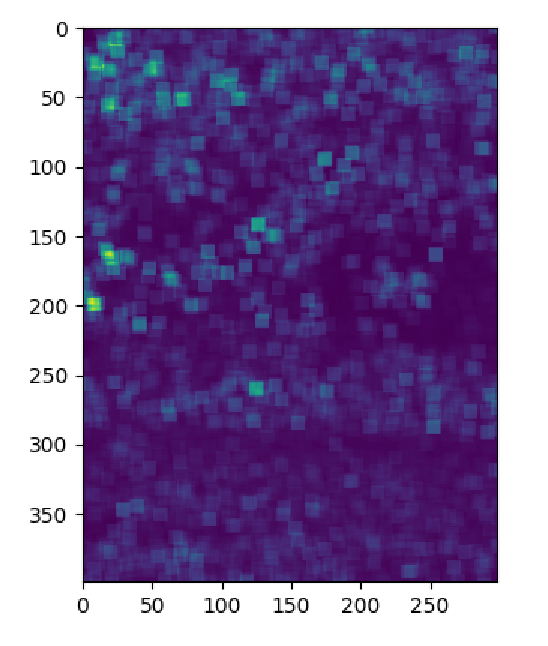
\includegraphics[width=\textwidth]{Bilder/MSE_Bilder/cropped/kernel10_tent_256_0.007_m64_G.eps}
%     \caption{TE}
%     \label{MSE256TE}
%   \end{subfigure}\hfil
%   \begin{subfigure}{.25\textwidth}
%     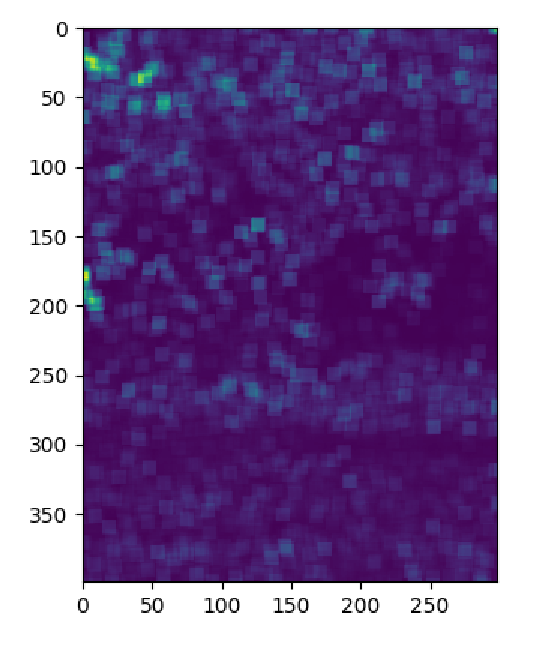
\includegraphics[width=\textwidth]{Bilder/MSE_Bilder/cropped/kernel10_magnitude_256_0.007_m0.0001_G.eps}
%     \caption{ME}
%     \label{MSE256ME}
%   \end{subfigure}\hfill
%   \caption{Local MSE-Loss for $d=256$, green channel, brighter colors represent larger values}
%   \label{MSE256}
% \end{figure}

% In the loss map for PE with $d=256$ the giraffe stands out. This can be attributed to the encoding losing resemblance in the neighborhood of each pixel. This can be interpreted as the encodings of neighboring coordinates lacking similarity which impedes generalization. Training pixels are unaffected by this problem causing the model to overfit.
% !TEX root = ../svrhm.tex
\section{Results}
Among the tested encodings TE and ME show the best results. For higher population sizes, PE achieves great results on the training set, but fails to generalize as seen in figure \ref{PE256}. TE and ME perform similarly to PE on the training set but exhibit better generalization.

\subsection*{Failure cases}
When using TE, it must be ensured that the tent functions have sufficient width. 
The slope $m$ must not exceed $d/4$, i.e. the tent width is at least $8/d$. 
Otherwise, mirroring artifacts occur as seen in figure \ref{TEartefact} as the neural network fails to distinguish between different input scalars that have similar repesentations. The same phenomenon happens with ME when setting $\sigma$ too small. 
When working with PE, large population sizes can lead to bad generalization. A more detailed analysis is given in appendix \ref{LocalMSE}. 
%PE mit hoher Dimension
%Spiegelartefakte bei Tent-Encoding
%Artefakte bei ME mit zu kleinem Sigma
\section{Conclusion}

Using population coding has proven to vastly increase the capability to learn high frequency dependencies between input and output of a neural network. Across encoding schemes, a correlation between population size and resolution of the learned function can be observed, with diminishing returns for large populations. 

In order to avoid overfitting, small differences in input values must not lead to drastic changes in the encoded representation. This is demonstrated to be a problem for a class of commonly used position encoding methods, with other encoding schemes being less susceptible to this issue. 

Overall, Magnitude Encoding and Tent Encoding show the best results among the compared population coding schemes. 

An interesting prospect is the use of population coding to explicitly encode features inside a neural network. While a neural network can in theory learn these population coded features, this work is evidence that in practice it does not do so, at least not for the input layer.

Potential applications include late fusion models, as well as sequence models with low dimensional sequence samples, like audio waveforms and other time series data. In these scenarios using population coding on the input might drastically improve model performances.

\bibliographystyle{svrhm_2022}
\bibliography{my_bibliography}


%%%%%%%%%%%%%%%%%%%%%%%%%%%%%%%%%%%%%%%%%%%%%%%%%%%%%%%%%%%%

\newpage
\appendix


\section{Appendix}

\subsection{Plots}
\label{subsecPlots}
Figure \ref{Plots} shows visualizations of the four coding schemes. Figure \ref{PlotPE} shows Positional Encoding for $L=2$. Figure \ref{PlotFE} shows four sine and cosine waves with random parameters for \textbf{b}. Tent encoding in figure \ref{PlotTE} uses parameters $m=1$ and $L=5$. The gaussian curves in figure \ref{PlotME} are created with parameters $\sigma=0.2$ and $L=5$.
\begin{figure}[!h]
  \begin{subfigure}{.5\textwidth}
  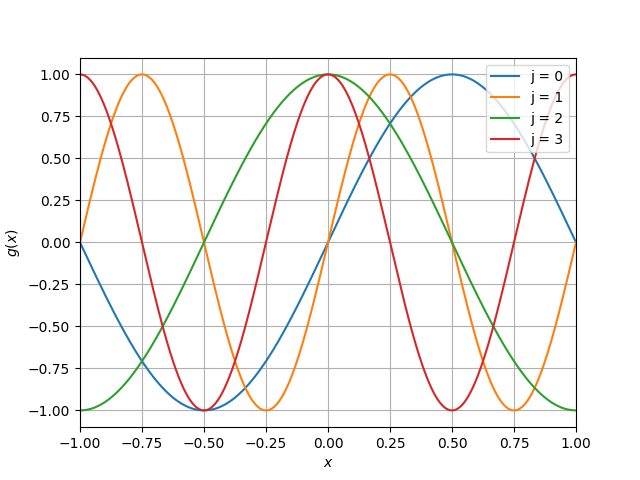
\includegraphics[width=\textwidth]{Bilder/plot_positional.png}
  \caption{Positional Encoding}
  \label{PlotPE}
\end{subfigure}
\begin{subfigure}{.5\textwidth}
  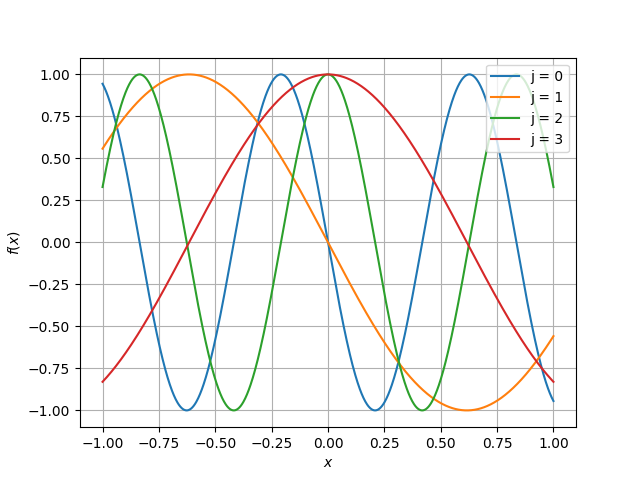
\includegraphics[width=\textwidth]{Bilder/plot_fourier.png}
  \caption{Fourier Feature Mapping}
  \label{PlotFE}
\end{subfigure}
\begin{subfigure}{.5\textwidth}
  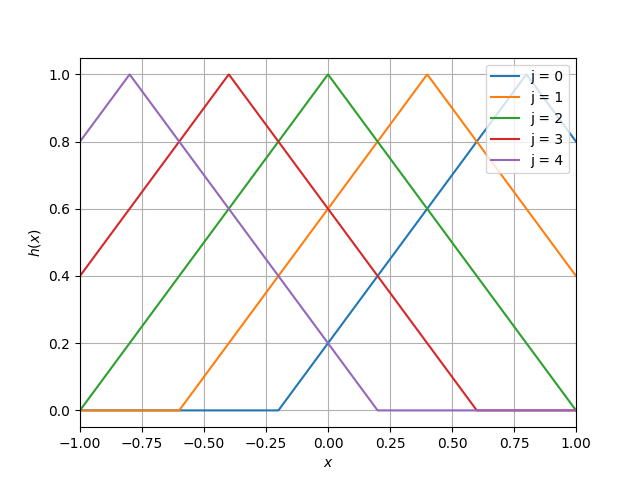
\includegraphics[width=\textwidth]{Bilder/plot_tent.png}
  \caption{Tent Encoding}
  \label{PlotTE}
\end{subfigure}
\begin{subfigure}{.5\textwidth}
  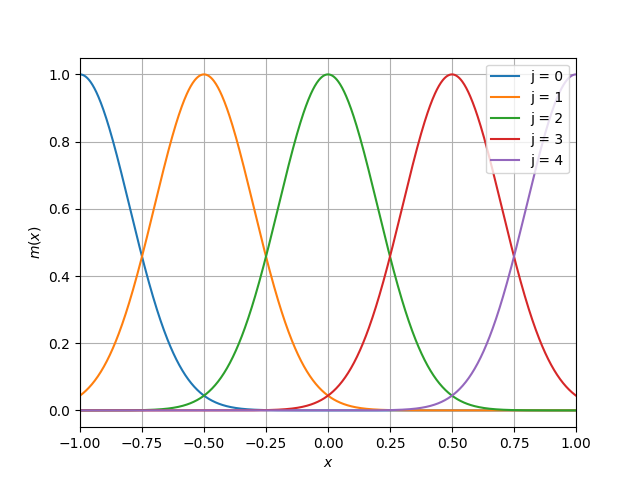
\includegraphics[width=\textwidth]{Bilder/plot_magnitude_varianz.png}
  \caption{Magnitude Encoding}
  \label{PlotME}
\end{subfigure}
\caption{Visualization of the four coding schemes.}
\label{Plots}
\end{figure}

\subsection{Local MSE-Loss}
\label{LocalMSE}
To localize the contribution to the overall reconstruction loss the mean squared error is calculated over a sliding $10\times10$-window on a single channel. The resulting loss map is shown in figure \ref{MSE256}.
% \begin{figure}
%   \begin{subfigure}{.25\textwidth}
%     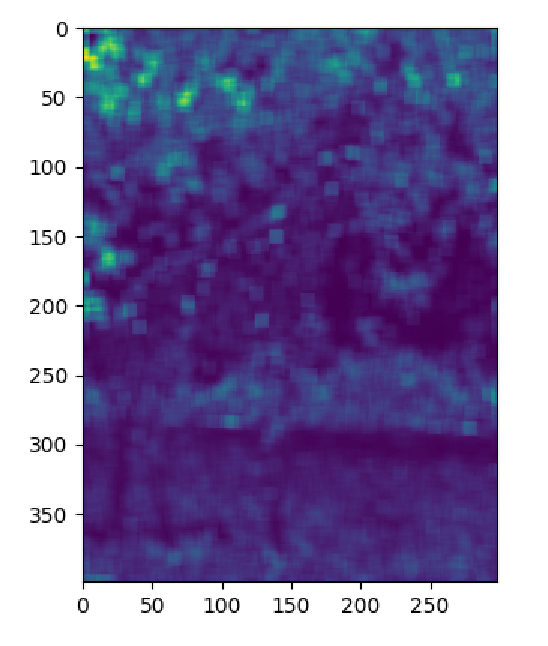
\includegraphics[width=\textwidth]{Bilder/MSE_Bilder/cropped/kernel10_positional_16_0.003_m0_G.eps}
%     \caption{PE}
%     \label{MSE16PE}
%   \end{subfigure}\hfil
%   \begin{subfigure}{.25\textwidth}
%     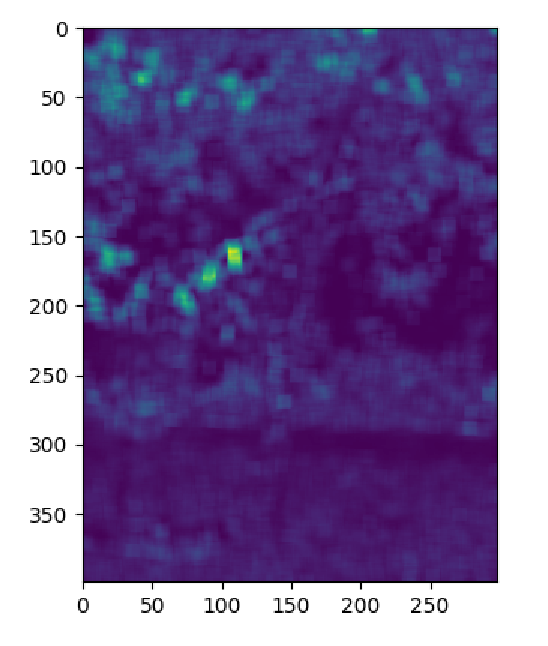
\includegraphics[width=\textwidth]{Bilder/MSE_Bilder/cropped/kernel10_fourier_16_0.01_G.eps}
%     \caption{FFM}
%     \label{MSE16FFM}
%   \end{subfigure}\hfil
%   \begin{subfigure}{.25\textwidth}
%     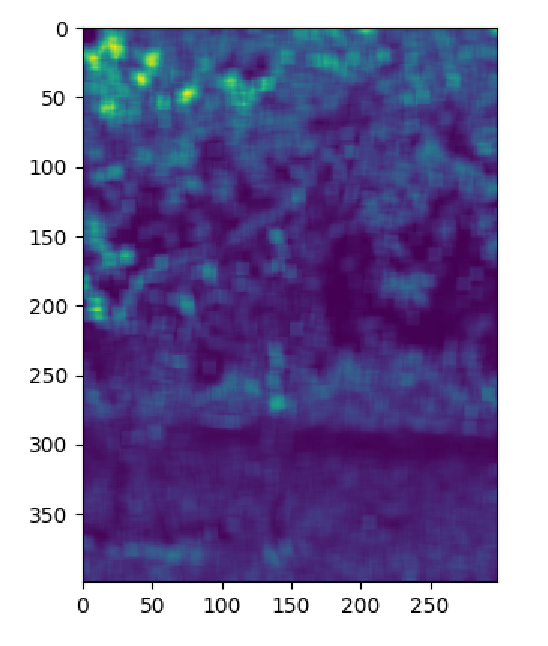
\includegraphics[width=\textwidth]{Bilder/MSE_Bilder/cropped/kernel10_tent16_m4_0.00667_G.eps}
%     \caption{TE}
%     \label{MSE16TE}
%   \end{subfigure}\hfil
%   \begin{subfigure}{.25\textwidth}
%     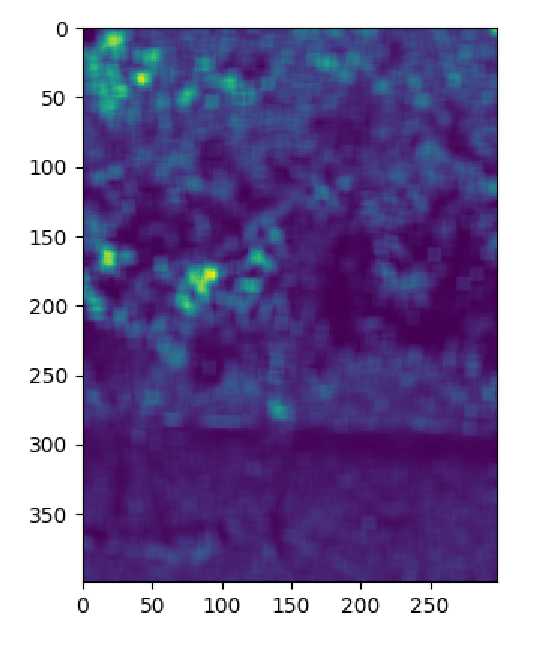
\includegraphics[width=\textwidth]{Bilder/MSE_Bilder/cropped/kernel10_magnitude_16_0.007_m0.05_G.eps}
%     \caption{ME}
%     \label{MSE16ME}
%   \end{subfigure}\hfill
%   \caption{Local MSE-Loss for $d=16$, green channel, brighter colors represent larger values}
%   \label{MSE16}
% \end{figure}

All of the encoding approaches lead to better image reconstruction than no enconding at all. The image background exhibits a higher loss than objects in the foreground. This may be attributed to the background features having higher entropy, i.e. higher information content. 

\begin{figure}[!h]
  \begin{subfigure}{.2\textwidth}
    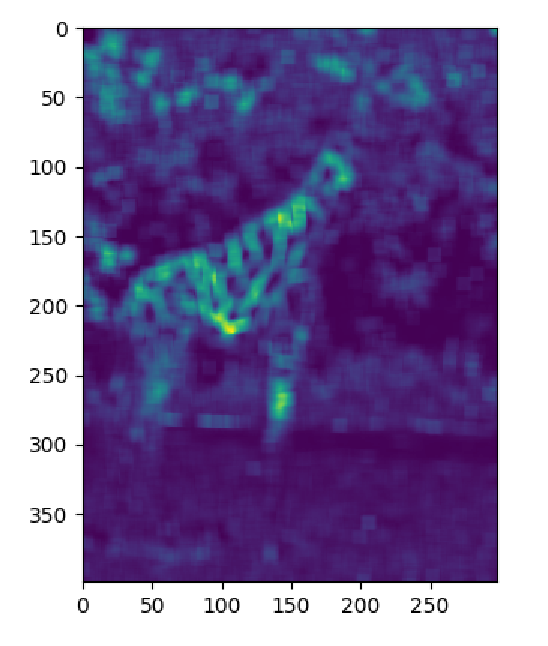
\includegraphics[width=\textwidth]{Bilder/MSE_Bilder/cropped/kernel10_scale_0.003_G.eps}
    \caption{No encoding}
    \label{MSE256Scale}
  \end{subfigure}\hfill
  \begin{subfigure}{.2\textwidth}
    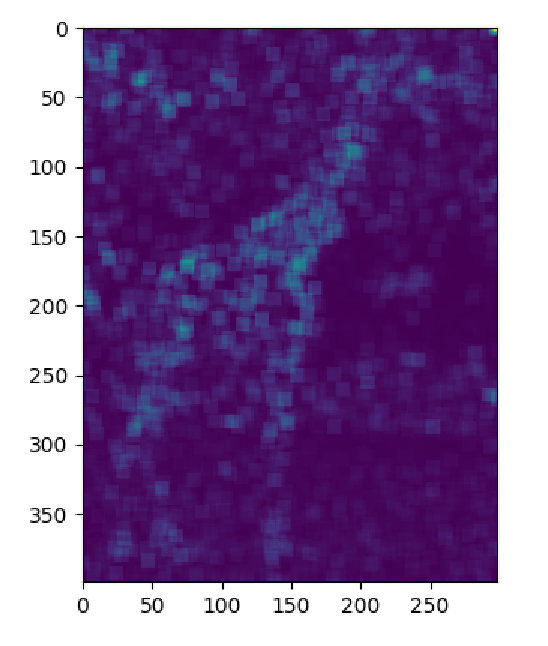
\includegraphics[width=\textwidth]{Bilder/MSE_Bilder/cropped/kernel10_positional_256_0.003_m0_G.eps}
    \caption{PE}
    \label{MSE256PE}
  \end{subfigure}\hfil
  \begin{subfigure}{.2\textwidth}
    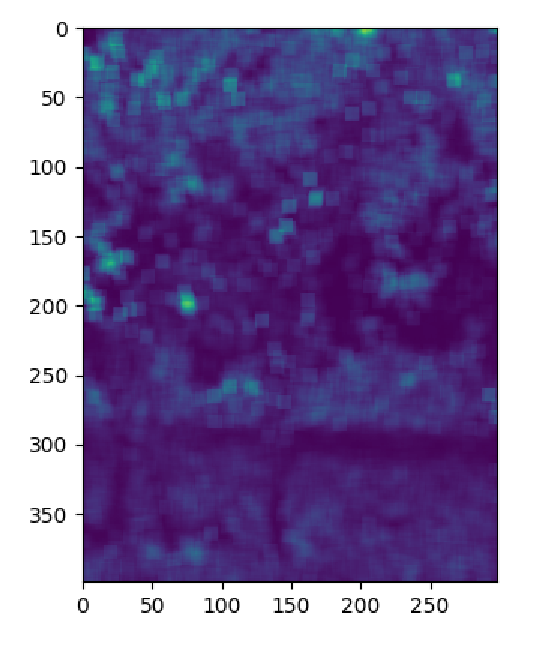
\includegraphics[width=\textwidth]{Bilder/MSE_Bilder/cropped/kernel10_fourier_256_0.01_G.eps}
    \caption{FFM}
    \label{MSE256FFM}
  \end{subfigure}\hfil
  \begin{subfigure}{.2\textwidth}
    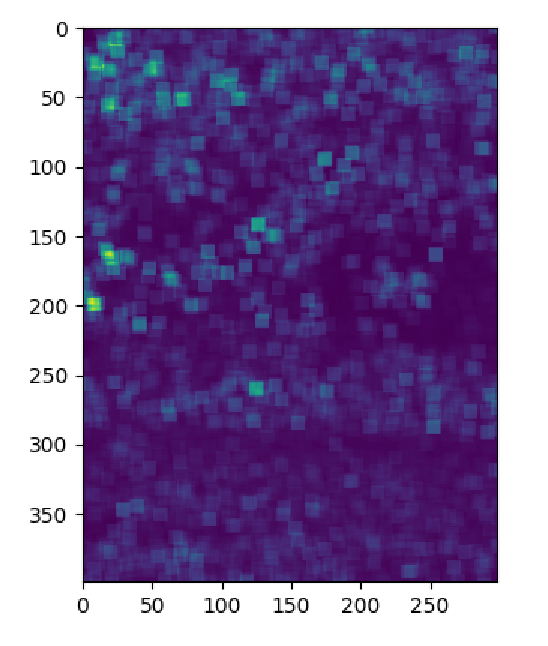
\includegraphics[width=\textwidth]{Bilder/MSE_Bilder/cropped/kernel10_tent_256_0.007_m64_G.eps}
    \caption{TE}
    \label{MSE256TE}
  \end{subfigure}\hfil
  \begin{subfigure}{.2\textwidth}
    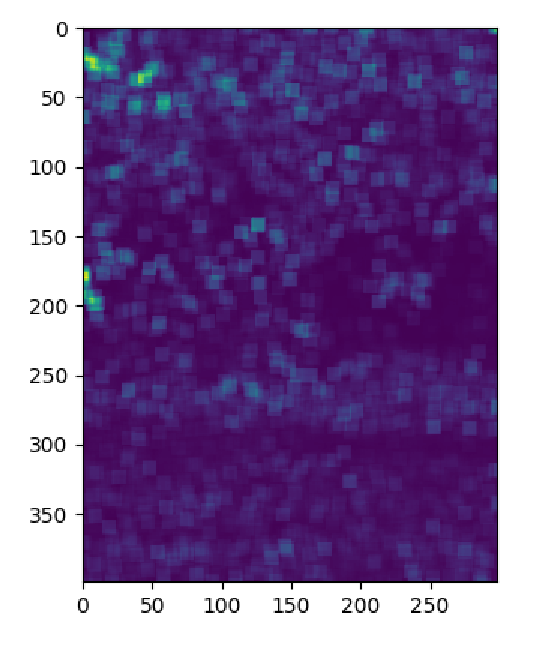
\includegraphics[width=\textwidth]{Bilder/MSE_Bilder/cropped/kernel10_magnitude_256_0.007_m0.0001_G.eps}
    \caption{ME}
    \label{MSE256ME}
  \end{subfigure}\hfill
  \caption{Local MSE-Loss for $d=256$, green channel, brighter colors represent larger values.}
  \label{MSE256}
\end{figure}

In the loss map for PE with $d=256$ the giraffe stands out. This can be attributed to the encoding losing resemblance in the neighborhood of each pixel. This can be interpreted as the encodings of neighboring coordinates lacking similarity which impedes generalization. Training pixels are unaffected by this problem causing the model to overfit.

\end{document}